\section{Multijets background}
\label{sec:qcd} 

This section describes the data driven estimate
of the contribution of QCD multijet events to the 
background in both the \eejj~and \enujj~channels.
In both channels, QCD multijet events may only contribute
to the background if one or more jets is 
misidentified as a HEEP electron.
Section \ref{sec:qcdDescription} gives an overview of the method for this estimate.
Section \ref{sec:qcdFakeRateCalc} describes the rates with which jets can be
misidentified as a HEEP electron.
Section \ref{sec:qcdEstimate} describes how these misidentification rates
are applied in both the \eejj~and \enujj~channels, 
and Section \ref{sec:qcdClosureTest} describes a closure test
used as a cross check for this background estimate.

\subsection{Method}
\label{sec:qcdDescription}

The QCD multijet background in both \eejj~and \enujj~channels 
is determined from data using a fake rate method.
Two data samples, "loose \eejj" and "loose \enujj", 
dominated by QCD multijet events are selected.  In both samples, electrons are 
required to pass "loose" identification requirements instead of the "tight" HEEP selection 
described in Section~\ref{sec:id-electron}.
The other jet and \MET~requirements and kinematic 
selection criteria remain unchanged.

The number of QCD multijet events in the \eejj~sample, $N_{eejj}^{QCD}$, 
at a given stage of the selection is estimated by Equation~\ref{eqn:qcdFakeRate-eejj}:
\begin{equation}
  N_{eejj}^{QCD} = \sum_{\text{loose } eejj \text{ events in data}} P(e_{1\text{, tight}} | e_{\text{1, loose}}: p_{T}, \eta) \cdot P(e_{2\text{, tight}} | e_{\text{2, loose}}: p_{T}, \eta) \quad
  \label{eqn:qcdFakeRate-eejj}
\end{equation}
Similarly, the number of QCD multijet events in the \enujj~sample, $N_{e \nu jj}^{QCD}$, 
at a given stage of the selection is estimated by Equation~\ref{eqn:qcdFakeRate-enujj}:
\begin{equation}
  N_{e \nu jj}^{QCD} = \sum_{\text{loose } e \nu jj \text{ events in data}} P(e_{\text{tight}} | e_{\text{loose}}: p_{T}, \eta) \quad
  \label{eqn:qcdFakeRate-enujj}
\end{equation}
where 
$e_{\text{loose}}$ is a GSF electron passing loose electron identification      
criteria described in Table~\ref{tab:qcdSelection}, 
$e_{\text{tight}}$ is an electron passing the HEEP ID and isolation criteria 
described in Section~\ref{sec:id-electron}, and 
$P(e_{\text{loose}} | e_{\text{tight}}: p_{T}, \eta)$ is the probability, or fake
rate, that a loose electron $e_{\text{loose}}$ passes the HEEP ID and isolation requirements.  
The sum is performed over all of the events in the loose \eejj~and \enujj~data samples that
pass the event selection.  

The events in the loose \enujj~and \eejj~samples are selected online by
prescaled single photon triggers with 
different \et~thresholds (depending on the run range), as shown in Table \ref{tab:qcd-trig}.
These triggers require an energy cluster in the ECAL with a reconstructed $\et$ greater than
a threshold in GeV indicated by the number after the word {\tt Photon} in the trigger name.
In addition, the triggers in Table \ref{tab:qcd-trig} with the word {\tt CaloIdVL} in their name 
also require the absence of significant energy deposits in the HCAL cells directly behind the ECAL cluster
(\HoE$ < 0.15$ for electrons in the EB, \HoE$ < 0.10$ for electrons in the EE)
and the shape of the ECAL cluster must be consistent with the shape of clusters typically produced by electrons and photons
(\SigmaiEtaiEta$ < 0.024$ for electrons in the EB, \SigmaiEtaiEta$ < 0.040$ for electrons in the EE).

Depending on the \et~of the triggered photon, each event passing the loose
\eejj~or \enujj~selection is reweighted in the sum of Equations~\ref{eqn:qcdFakeRate-eejj} 
and~\ref{eqn:qcdFakeRate-enujj} with a weight equal to the lowest trigger prescale among 
the single photon triggers that fired in that event.
The \et~threshold of the lowest single photon trigger ({\verb HLT_Photon30_CaloIdVL })
is 30~\GeV.  This value is 10~\GeV~below the electron \pt~used in preselection for both analyses:
enough to avoid any trigger threshold bias.

\begin{table}
  \begin{center}
    \begin{tabular}{l|c|c}
      Variable & Barrel (EB) criterion & Endcap (EE) criterion \\
      \hline
      \hline
      $\sigma_{i\eta i\eta}$ & $<$ 0.013 & $<$ 0.034 \\
      $H/E$ & $<$ 0.15 &  $<$ 0.1 \\
    \end{tabular}
    \caption{Loose identification criteria for gsf electrons needed for the QCD multijet background estimation.
      These criteria are used to select the loose \eejj~and \enujj~samples.  The variables listed in the leftmost
      column are defined in Section \ref{sec:id-electron}.}
    \label{tab:qcdSelection}
  \end{center}
\end{table}

\begin{table}
  \begin{center}
    % \scriptsize
    \begin{tabular}{l|c|c} 
      HLT path & Run number range & Effective \Lint (pb$^{-1}$) \\ 
      \hline
      \hline
      \verb HLT_Photon30_CaloIdVL_v1 & 160431--161176 & 0.145661  \\ 
      \verb HLT_Photon30_CaloIdVL_v2 & 161217--163261 & 0.341693  \\ 
      \verb HLT_Photon30_CaloIdVL_v3 & 163270--163869 & 0.778178  \\ 
      \verb HLT_Photon30_CaloIdVL_v4 & 165088--165633 & 0.441692  \\ 
      \verb HLT_Photon30_CaloIdVL_v5 & 165970--166967 & 0.573131  \\ 
      \verb HLT_Photon30_CaloIdVL_v6 & 167039--173198 & 0.909814  \\ 
      \verb HLT_Photon30_CaloIdVL_v7 & 173236--173692 & 0.537542  \\ 
      \verb HLT_Photon30_CaloIdVL_v8 & 175860--180252 & 1.176     \\ 
      \hline
      \verb HLT_Photon50_CaloIdVL_v1 & 165088--165633 & 1.734   \\ 
      \verb HLT_Photon50_CaloIdVL_v2 & 165970--166967 & 2.414   \\ 
      \verb HLT_Photon50_CaloIdVL_v3 & 167039--173198 & 5.266   \\ 
      \verb HLT_Photon50_CaloIdVL_v4 & 173236--180252 & 10.63 \\
      \hline
      \verb HLT_Photon75_CaloIdVL_v1 & 160431--161176 & 6.111  \\
      \verb HLT_Photon75_CaloIdVL_v2 & 161217--163261 & 40.565 \\
      \verb HLT_Photon75_CaloIdVL_v3 & 163270--163869 & 168.23 \\
      \verb HLT_Photon75_CaloIdVL_v4 & 165088--165633 & 24.128 \\
      \verb HLT_Photon75_CaloIdVL_v5 & 165970--166967 & 14.116 \\
      \verb HLT_Photon75_CaloIdVL_v6 & 167039--173198 & 32.136 \\
      \verb HLT_Photon75_CaloIdVL_v7 & 173236--180252 & 49.056 \\
      \hline
      \verb HLT_Photon90_CaloIdVL_v1 & 165088--165633 & 46.065  \\ 
      \verb HLT_Photon90_CaloIdVL_v2 & 165970--166967 & 28.232  \\ 
      \verb HLT_Photon90_CaloIdVL_v3 & 167039--173198 & 64.592  \\ 
      \verb HLT_Photon90_CaloIdVL_v4 & 173236--180252 & 163.279 \\ 
      \hline
      \verb HLT_Photon125_v1 & 165088--165633 & 136.382 \\ 
      \verb HLT_Photon125_v2 & 165970--166967 & 535.17  \\ 
      \hline                                           
      \verb HLT_Photon135_v1 & 167039--173198 & 1107.0   \\ 
      \verb HLT_Photon135_v2 & 173236--180252 & 2958.0  \\ 
      \hline                                           
      \verb HLT_Photon400_v1 & 167039--173198 & 1107.0  \\ 
      \verb HLT_Photon400_v2 & 173236--180252 & 2958.0  \\ 
    \end{tabular}
    \caption{Single photon HLT paths used for the QCD multijet background estimation.}
    \label{tab:qcd-trig}
  \end{center}
\end{table}

\subsection{Fake rate calculation}
\label{sec:qcdFakeRateCalc}

The fake rate, $P(e_{\text{tight}} | e_{\text{loose}}: p_{T}, \eta)$, is 
defined as the ratio between the number of HEEP electrons, $N_{e, \text{tight}}$,        
and the number of loose electrons, $N_{e, \text{loose}}$ identified with the criteria listed in
Table~\ref{tab:qcdSelection}, in a sample of events in data passing the 
following selection criteria:

\begin{enumerate}
\item The event must fire a single photon trigger, as described in Table \ref{tab:qcd-trig}
\item There must be exactly one loose electron, selected using the criteria described in Table \ref{tab:qcdSelection}
\item There must be $N_{\text{jet}}$ or more jets with $p_{T} > 40$ \GeV, with $N_{\text{jet}}$ equal to 0, 1, 2, or 3
\item $\Delta R(e_{\text{loose}}, \text{jets}) > 0.7$
\item \MET $< 30$~\GeV
\end{enumerate}

The requirements of exactly one loose electron and \MET~reduce
the contamination of real electrons in the sample from $\PZz \rightarrow ee$
and $W \rightarrow e\nu$ events.
The fake rates are calculated for the EB and for two separate regions of the EE
($|\eta| < 2.0$ and $|\eta| > 2.0$). In addition, each set of fake rates
is obtained for three different jet multiplicity requirements, as described 
in cut number 3, above.  The contamination of real electrons in both
$N_{e, \text{tight}}$ and $N_{e, \text{loose}}$ is subtracted from the data using
MC predictions. The MC samples are normalized using the cross sections listed in 
Section~\ref{sec:mc-samples}. The MC-corrected fake rate for the  
$N_{\text{jet}} \geq 2$ case is shown in Figure~\ref{fig:fakeRateNjetGtTwo} as a 
function of the loose electron \pt, separately for the barrel and the two endcap regions.  

Following the approach of the Z'$\rightarrow \mbox{ee}$ analysis~\cite{zprime-2011}, each fake rate is fit 
with a first-degree polynomial in the region $\mbox{\pt} < 100$~\GeV~and 
a zero-degree polynomial in the region $\mbox{\pt} > 100$~\GeV.
The fit results are reported in Table~\ref{tab:fakeRates} for the four cases under consideration:
$N_{\text{jet}} \geq 0$, $N_{\text{jet}} \geq 1$, $N_{\text{jet}} \geq 2$, and
$N_{\text{jet}} \geq 3$.  The value of the fake rate decreases with increasing jet multiplicity. 
The fake rates that are used for the \eejj~and \enujj~QCD multijet background estimation 
are from the $N_{\text{jet}} \geq 2$ case.

\begin{figure}
  \centering
  \begin{tabular}{c}
    \resizebox{14cm}{!}{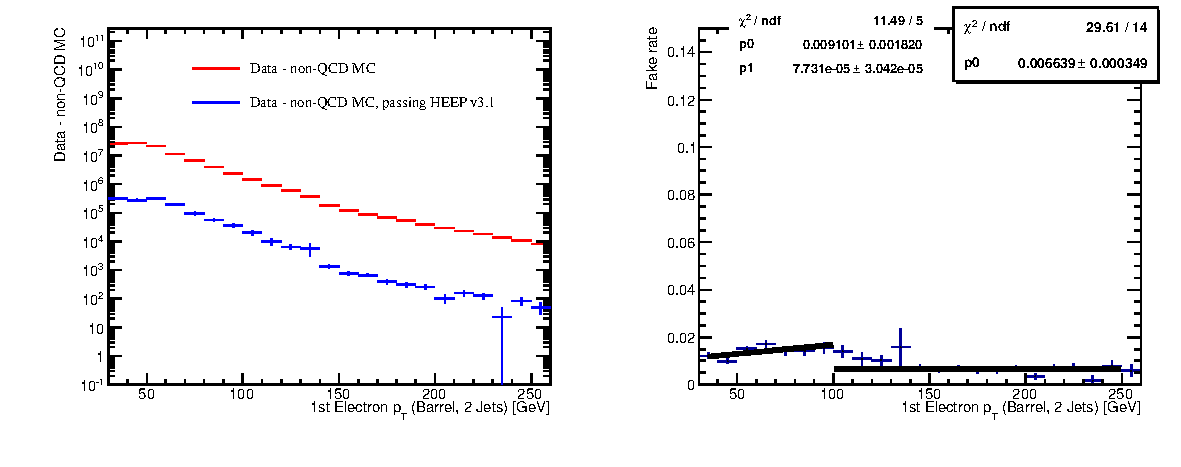
\includegraphics {tex/analysis/backgrounds/fig/Bar_2Jet_Pt1stEle_PAS.pdf} } \\
    \resizebox{14cm}{!}{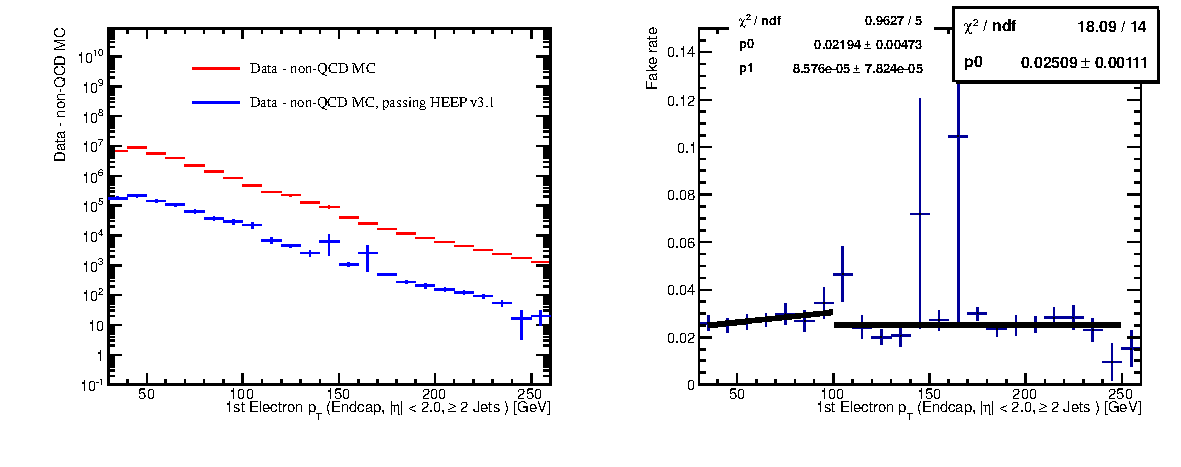
\includegraphics {tex/analysis/backgrounds/fig/End1_2Jet_Pt1stEle_PAS.pdf}} \\
    \resizebox{14cm}{!}{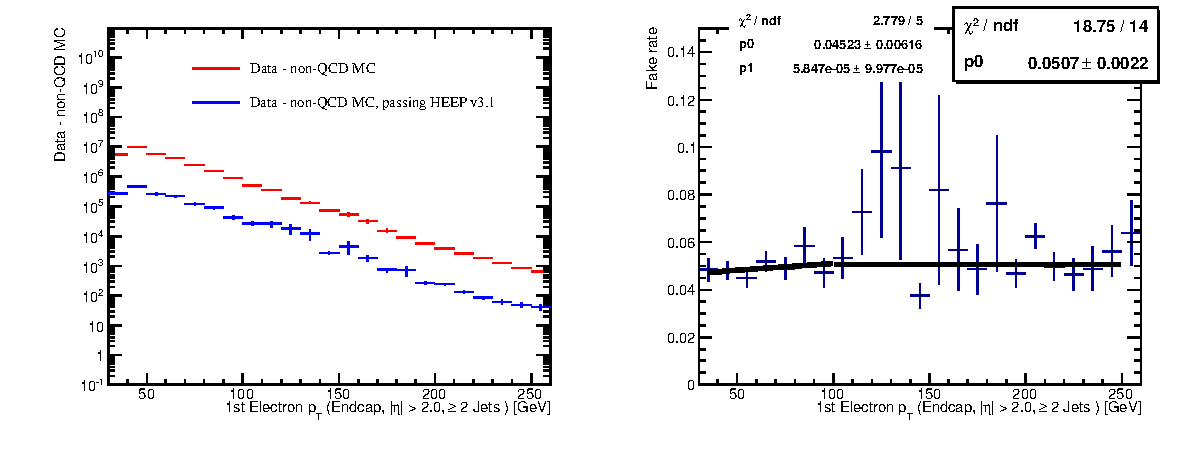
\includegraphics {tex/analysis/backgrounds/fig/End2_2Jet_Pt1stEle_PAS.pdf}} \\
  \end{tabular}
  \caption{The \pt~distribution of the "loose" and "tight" electrons in the fake rate sample (left) and 
    the corresponding fitted fake rate vs electron \pt~(right) for selected events with $N_{\text{jet}} \geq 2$. 
    The results are shown for the barrel and the two endcap regions. 
    The non-QCD contribution is subtracted from the electron \pt~distributions.}
  \label{fig:fakeRateNjetGtTwo}
\end{figure}   

\begin{table}
  \small
  \begin{center}
    \begin{tabular}{l|c|c|c}
      Selection & $p_{0}$ & $p_{1}$ & $p_{2}$ \\ 
      \hline 
      \hline 
      inclusive, barrel & 2.301e-02 $\pm$ 1.745e-03 & -6.570e-05 $\pm$ 2.888e-05 & 7.574e-03 $\pm$ 3.228e-04 \\ 
      inclusive, endcap ($|\eta| < 2.0$ ) & 4.060e-02 $\pm$ 3.991e-03 & -1.005e-04 $\pm$ 6.649e-05 & 2.680e-02 $\pm$ 1.005e-03 \\ 
      inclusive, endcap ($|\eta| > 2.0$ ) & 6.313e-02 $\pm$ 5.103e-03 & -1.033e-04 $\pm$ 8.795e-05 & 5.270e-02 $\pm$ 2.020e-03 \\ 
      \hline 
      1 jet, barrel & 1.783e-02 $\pm$ 1.595e-03 & 3.067e-06 $\pm$ 2.721e-05 & 7.585e-03 $\pm$ 3.227e-04 \\ 
      1 jet, endcap ($|\eta| < 2.0$ ) & 3.673e-02 $\pm$ 3.837e-03 & -4.838e-05 $\pm$ 6.475e-05 & 2.681e-02 $\pm$ 1.005e-03 \\ 
      1 jet, endcap ($|\eta| > 2.0$ ) & 6.020e-02 $\pm$ 4.995e-03 & -6.142e-05 $\pm$ 8.666e-05 & 5.270e-02 $\pm$ 2.020e-03 \\ 
      \hline 
      2 jets, barrel & 9.101e-03 $\pm$ 1.820e-03 & 7.731e-05 $\pm$ 3.042e-05 & 6.639e-03 $\pm$ 3.494e-04 \\ 
      2 jets, endcap ($|\eta| < 2.0$ ) & 2.194e-02 $\pm$ 4.734e-03 & 8.576e-05 $\pm$ 7.824e-05 & 2.509e-02 $\pm$ 1.109e-03 \\ 
      2 jets, endcap ($|\eta| > 2.0$ ) & 4.523e-02 $\pm$ 6.162e-03 & 5.847e-05 $\pm$ 9.977e-05 & 5.070e-02 $\pm$ 2.197e-03 \\ 
      \hline 
      3 jets, barrel & 1.538e-03 $\pm$ 2.476e-03 & 1.224e-04 $\pm$ 4.192e-05 & 4.753e-03 $\pm$ 4.328e-04 \\ 
      3 jets, endcap ($|\eta| < 2.0$ ) & 8.950e-04 $\pm$ 6.942e-03 & 3.409e-04 $\pm$ 1.170e-04 & 2.531e-02 $\pm$ 1.292e-03 \\ 
      3 jets, endcap ($|\eta| > 2.0$ ) & 1.863e-02 $\pm$ 8.961e-03 & 2.997e-04 $\pm$ 1.399e-04 & 4.799e-02 $\pm$ 2.416e-03 \\ 
    \end{tabular}   
    \caption{
      Fake rates and relative fit parameters. \\ 
      The fit functions are: 
      $f(\mbox{\pt}) = p_{0} + p_{1} \cdot \mbox{\pt}$ for $\mbox{\pt}<100$, and 
      $f(\mbox{\pt}) = p_{2}$ for $\mbox{\pt} > 100$.
    }
    \label{tab:fakeRates}
  \end{center}
\end{table}

\subsection{Background estimate}
\label{sec:qcdEstimate}
At each step of the \eejj~and \enujj~selections, the shape of the kinematic
distributions and the normalization of the QCD multijet background are estimated with the method
described in Section~\ref{sec:qcdDescription}, using Equations~\ref{eqn:qcdFakeRate-eejj} and~\ref{eqn:qcdFakeRate-enujj}.  
Tables~\ref{tab:eejjFinalSelection} and~\ref{tab:enujjFinalSelection} report the QCD multijet contribution at different stages
of the event selection for each analysis using the $N_{\text{jet}} \geq 2$ fake rates. 
After the final selection, the QCD multijet contribution is \QCDcontributionINeejj~(\QCDcontributionINenujj) 
of the total background in the \eejj~(\enujj) channels for leptoquark masses around the current reach of this search.  

\subsection{Closure test}
\label{sec:qcdClosureTest}
A closure test is performed in order to validate the QCD multijet background 
estimation using the fake rate method. This closure test uses a control sample of 
QCD multijet events (with a contamination from non-QCD processes of \ContaminationAtQCDForClosureTestLooseLoose)
selected by the following requirements:
\begin{enumerate}
\item the event must fire a single photon trigger, as described in Table~\ref{tab:qcd-trig}
\item there must be exactly two loose electrons, selected using the criteria described in Table~\ref{tab:qcdSelection}
\item there must be at least one jet with $p_{T} > 40$~\GeV
\item $\Delta R(e_{\text{loose}}, \text{jets}) > 0.7$
\item $M_{ee} > 110$~\GeV, to reduce contamination from $\mbox{\PZz} \rightarrow \mbox{ee}$ events
\item $\st > 200$~\GeV, where \st~is defined as the scalar sum of the two loose electrons and the leading (in \pt) jet
\end{enumerate}

A prediction is made of how many of these events will have one electron passing the HEEP
identification and isolation criteria described in Section~\ref{sec:id-electron}, 
$N_{\text{loose }e\text{, tight }e\text{, }j}^{QCD, pred.}$, using the $N_{\text{jet}} \geq 1$ 
fake rates calculated in Section~\ref{sec:qcdFakeRateCalc} and following a similar procedure 
as the one described in the previous sections:  
\begin{equation}
  \label{eqn:qcdClosureTest}
  N_{\text{loose }e\text{, tight }e\text{, }j}^{QCD, pred.} = \sum_{\text{loose }e,\text{ loose e, }j\text{ events}} P(e_{1\text{, tight}} | e_{\text{1, loose}}: p_{T}, \eta) + P(e_{2\text{, tight}} | e_{\text{2, loose}}: p_{T}, \eta)
\end{equation}
This prediction is then compared with the actual number 
of events in data where one of the two loose electrons also passes the tight selection criteria, $N_{\text{loose }e\text{, tight }e\text{, }j}^{QCD, actual}$.
In this comparison, the contribution of \ContaminationAtQCDForClosureTestLooseTight  from non-QCD multijet processes 
contaminating the actual "$\text{loose }e\text{, tight }e\text{, }j$" data sample is subtracted using an estimate from 
MC (the samples are normalized using the cross sections listed in Section~\ref{sec:mc-samples}). 

The predicted and actual values of "$\text{loose }e\text{, tight }e\text{, }j$"  events 
corresponding to \lumi of data are: $N_{\text{loose }e\text{, tight }e\text{, }j}^{QCD, pred.} = \mbox{\NeventsLTJpred}$
and $N_{\text{loose }e\text{, tight }e\text{, }j}^{QCD, actual} = \mbox{\NeventsLTJactual}$ (the latter after MC subtraction). 
Statistical errors derived from the uncertainties of fake rate fit parameters, and the uncertainties on the MC predictions
used in the subtraction are included. The ratio between the two values is \RatioLTJpredVSactual.
If an \st~\footnote{\st~is defined as the scalar sum of the two loose electrons and the leading jet} cut of 450 GeV
is applied 
(corresponding to the lowest \st~cut applied in the \enujj~final selection), the values become 
$N_{\text{loose }e\text{, tight }e\text{, }j}^{QCD, pred.} = \mbox{\NeventsLTJpredSTCUT}$ and 
$N_{\text{loose }e\text{, tight }e\text{, }j}^{QCD, actual} = \mbox{\NeventsLTJactualSTCUT}$, 
and their ratio is \RatioLTJpredVSactualSTCUT. 
Therefore, an uncertainty of \QCDUncertEEjj~(\QCDUncertEnujj) is quoted 
on this method at final selection level for the \eejj~(\enujj) channel.
Figure~\ref{fig:closureTest} shows the distributions of electron and jet reconstructed quantities 
for "$\text{loose }e\text{, tight }e\text{, }j$" events.
The QCD multijet prediction using the fake rate method 
is compared with the actual data sample and an acceptable agreement is observed in both the shape 
and the normalization of the two samples within the quoted uncertainties.

\begin{figure}[htbp]
  \begin{center}
    \begin{tabular}{cc}
      \resizebox{7.5cm}{!}{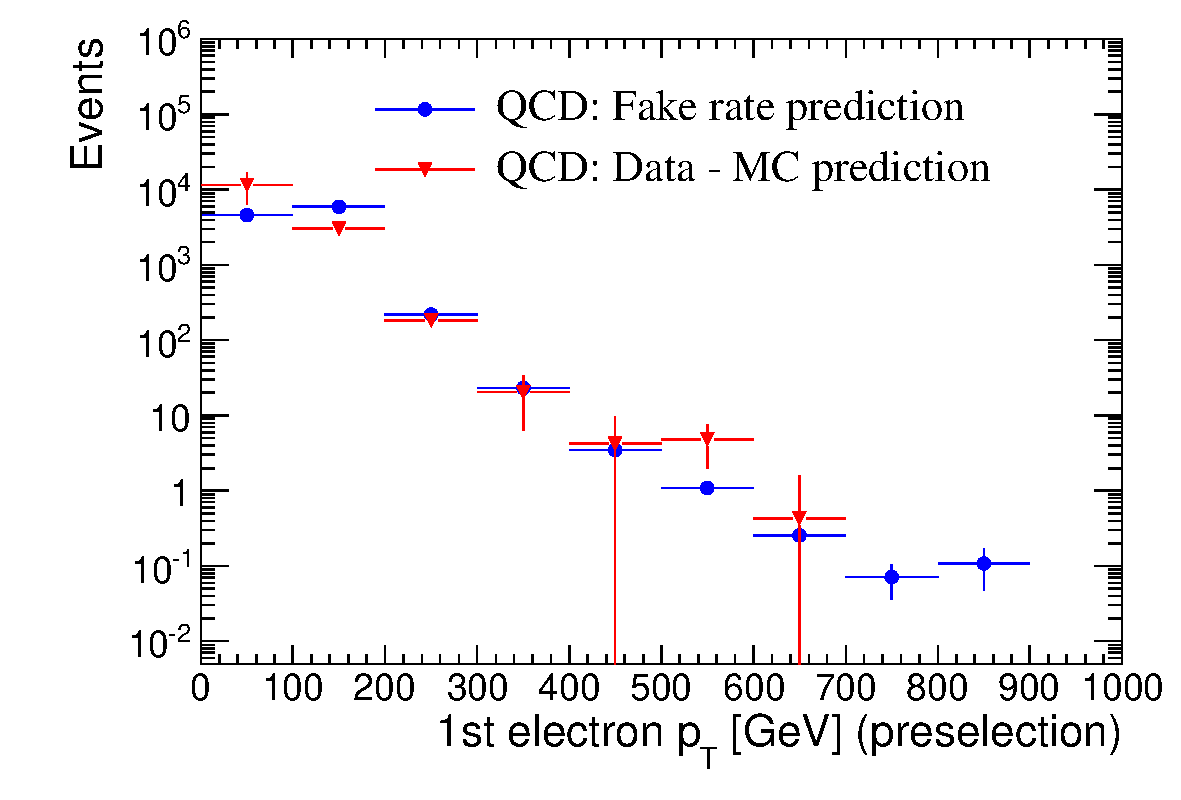
\includegraphics{tex/analysis/backgrounds/fig/Pt1stEle_PAS_closureTestQCD.pdf}} &
      \resizebox{7.5cm}{!}{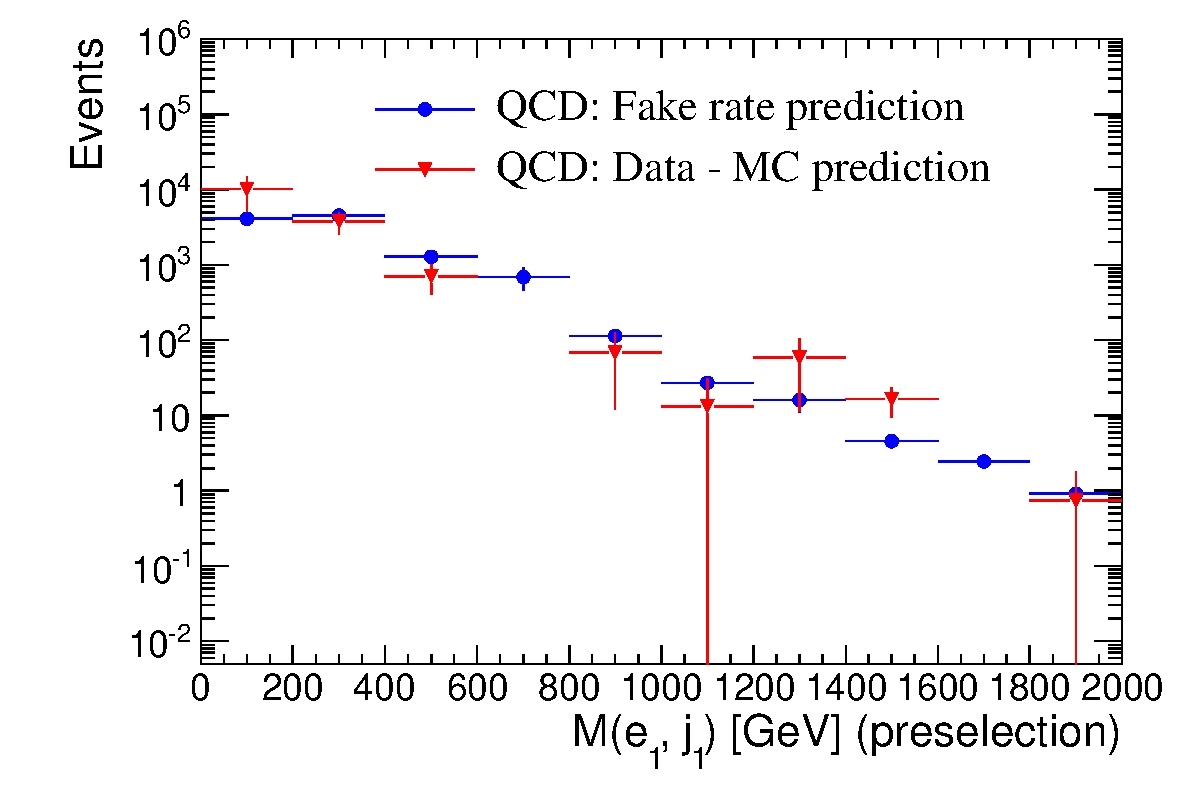
\includegraphics{tex/analysis/backgrounds/fig/Me1j1_PAS_closureTestQCD.pdf}} \\
      \resizebox{7.5cm}{!}{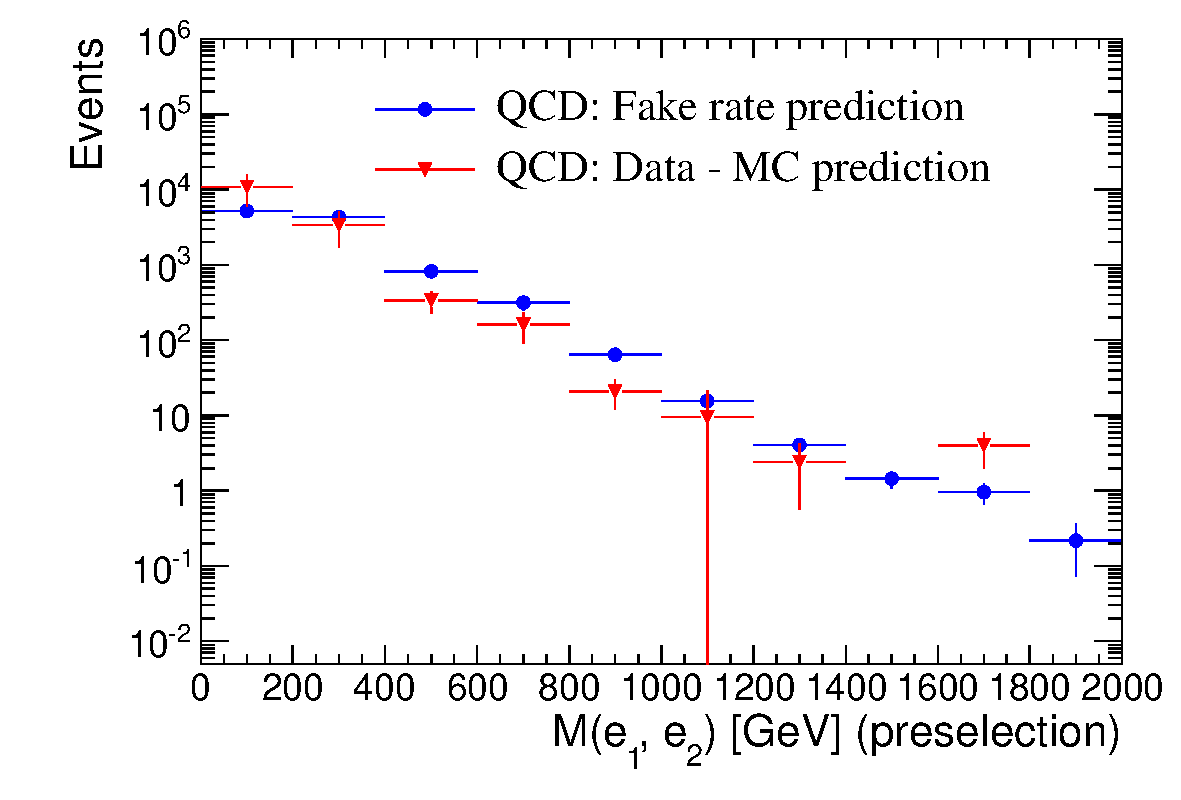
\includegraphics{tex/analysis/backgrounds/fig/Mee_PAS_closureTestQCD.pdf}} &
      \resizebox{7.5cm}{!}{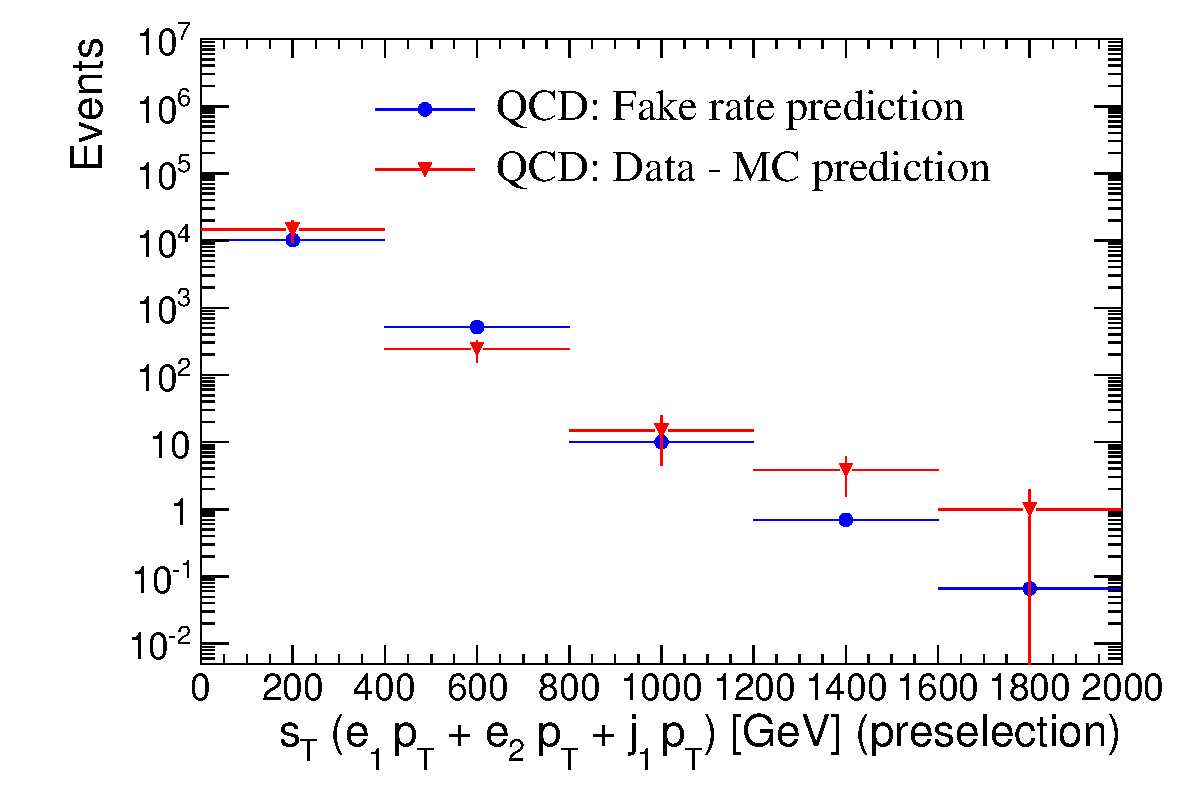
\includegraphics{tex/analysis/backgrounds/fig/sT_PAS_closureTestQCD.pdf}} \\
    \end{tabular}
    \caption{The leading electron \pt~(top left), \mej~(top right), 
      \mee (bottom left) and \st~(bottom right) distributions for 
      the "$\text{loose }e\text{, tight }e\text{, }j$" events. 
      The QCD multijet prediction using the fake rate method
      is compared with the actual data sample 
      (after the MC subtraction of non-QCD events 
      for the latter sample).
    }
    \label{fig:closureTest}
  \end{center}
\end{figure}   
